%\documentclass[12pt,preprint]{aastex}
\documentclass{emulateapj}
%\usepackage{apjfonts}
\usepackage{amsmath}
\usepackage{natbib}
\usepackage{graphicx}
\usepackage{bm}

\slugcomment{}

%% macros
\newcommand\da{\delta\!\alpha}
\newcommand\ks{\kappa_s}
\newcommand\ps{\phi_{\rm sub}}
\newcommand\mathbi[1]{\textbf{\em #1}}
\newcommand\rv{\bm r}
\newcommand\xv{\bm x}
\newcommand\uv{\bm u}
\newcommand\du{\delta\uv}
\newcommand\av{\bm \alpha}
\newcommand\dphi{\delta\phi}
\newcommand\dtau{\delta\tau}
\newcommand\avg[1]{\left\langle{#1}\right\rangle}
\newcommand\Rein{R_{\rm Ein}}
\newcommand\Sigcr{\Sigma_{\rm crit}}
\newcommand\tot{{\rm tot}}
\newcommand\mhat{{\hat m}}

\shorttitle{Inferring Time Delays in Strong Gravitational Lenses}
\shortauthors{Leonidas A.~Moustakas \& Andrew~Romero-Wolf}

\begin{document}

\title{Optimizing Observing Campaigns for Strong  Gravitational Lens Time Delays} 
\author{Leonidas A. Moustakas \& Andrew Romero-Wolf\altaffilmark{1}} 
\altaffiltext{1}{Jet Propulsion Laboratory, California Institute of
  Technology, 4800 Oak Grove Dr, M/S\,169-506, Pasadena, CA~~91109}

\begin{abstract}
  We report on a flexible and extendable inference technique for
  measuring the time delays between images in time-varying strong
  gravitational lenses, and for optimizing observational parameters to
  achieve a target time delay precision.  Robust time delays and
  meaningful estimates of the corresponding uncertainties are
  essential for using such time delays for several astrophysical
  applications, including estimating the Hubble constant, other
  cosmological parameters, or for constraining lens-galaxy structure
  or substructure properties. Quasar's optical light curves have been
  shown to be described well by a damped random walk behavior. We
  build a generative model of paired quasar light curves which are
  offset by a constant delay and magnitude, and build an inference
  process using the emcee Markov Chain Monte Carlo engine.  With this
  framework, we explore the problem of designing observational
  campaigns that will achieve time delay measurements at a specific
  threshold level.  We apply this approach to a notional \emph{Hubble}
  Space Telescope lens-monitoring experiment, to determine the
  observing campaign characteristics and photometric sensitivity that
  are required to secure a greater than 90\% probability of measuring
  a 1.5-day time delay to a combined random and systematic precision
  of better than one hour, a more than twenty-fold improvement of what
  is presently achieved.  We discuss the extensibility of this
  approach to other experimental designs, including from
  short-cadence, focused ground-based campaigns. 
\end{abstract}
 
\keywords{gravitational lensing --- cosmology: dark matter} 

\section{Introduction}

Gravitational lensing time delays are a promising tool for measuring
Hubble's constant \citep[$H_0$;][]{Refsdal1964a} as well as dark
energy cosmological parameters \citep{Coe2009b,Linder2011a,Treu2013a},
with compelling complementarity to other techniques
\citep{Weinberg2013a, Linder2015a}.  Indeed, there is presently
tension in the value for $H_0$ inferred by the \emph{Planck} cosmic
microwave background analysis \citep{Planck-Collaboration2014a,
  Planck-Collaboration2015a}, and the best-determined values derived
by state of the art modeling of gravitational lenses
\citep[e.g.][]{Suyu2013a, Suyu2014a}.

Such measurements depend on detailed modeling of often complex
gravitational environments and material along the line of sight
\citep[e.g.][]{Greene2013a, Schneider2013a}, but the foundation is the
time delay measurement itself, which depends on the details of the
observational campaign timing and duration, and the associated
photometric measurements of each individual image in a
lens. Substantial campaigns have been undertaken over the past ten or
more years \citep[e.g.][]{Eigenbrod2005a, Tewes2013a}, achieving time
delay precisions of approaching $\sim1$\,day\footnote{COSMOGRAIL
  webpage, http://http://cosmograil.org}.  To date, achieving time
delays with greater precision has been elusive
\citep[e.g.][]{Oguri2007a}, due in part by the difficulty of
coordinating observing campaigns with better than approximately
nightly cadence.

However, with cosmological measurement implications of much more
precise and better-characterized time delays, and their potential of
being used to infer properties of the dark matter substructure
expected to be contained within lensing galaxies
\citep[e.g.][]{Primack2009a, Xu2009a}, we are driven to understand how
to design and analyze observing campaigns that may achieve an order of
magnitude higher time delay precision than is currently typical
\citep{Keeton2009a, Linder2011a}.

This motivates us to develop a time delay measurement technique that
can be used both for analysis of existing data, but also for the
systematic study of tailored sets of observations and observational
characteristics, for optimal design of campaigns, tailored to the
needs of the desired scientific goals. Many techniques for
\emph{fitting} observations have been explored to date; see the
discussion in \citet{Dobler2015a} and \citet{Liao2015a}, for a
detailed review.  

Since the measurement of the time delay in the first strong
gravitational lens discovered, Q0957$+$561 \citep{Walsh1979a,
  Press1999a}, there have been many significant efforts to
systematically monitor time domain variations in multiply imaged
quasars, particularly in radio \citep[e.g.][]{Fassnacht1999a} and
optical wavelengths \citep[c.f.\ compilations in][]{Oguri2007a,
  Mosquera2011a}.  The near future shows great potential for both vast
numbers of poorly-measured time delays (with the Large Synoptic Survey
Telescope), and for exquisitely-measured time delays (e.g.\ using
focused Las Cumbres Observatory Global Telescope campaigns, the
\emph{Hubble} Space Telescope, or another space-based platform such as
the proposed Observatory for Multi-Epoch Gravitational Lens
Astrophysics, e.g.\ \citealt{Moustakas2009a}). In either scenario, we
wish to be in a position where one may determine precisely how to
achieve a \emph{desired} time delay precision with a specific level of
certainty.

In this work, we take advantage of a predictive model for the time
variations of quasar light curves, to set up a Bayesian inference
framework.  This is developed in Section~\ref{sec:tdanalysis}, based
on descriptions of simulated quasar light curve pairs for particular
observational conditions.  A notional experimental design is explored
in detail in Section~\ref{sec:experiment}, to demonstrate our
framework's application to achieving a desired time delay precision at
a high confidence of success.  We discuss the results, and extensions
of this methodology to other experiments in
Section~\ref{sec:discussion}.  All code is written in python, version
controlled via a github repository.

\section{Inference Analysis Framework}\label{sec:tdanalysis}

In this work, we concentrate on optical, radio-quiet quasars. The
variability in these types of objects has been shown to be consistent
with a damped random walk process, where the fluctuations have a
characteristic amplitude and decay time that correlate with the black
hole mass and luminosity \citep{Kelly2009a}.  We will call these the
``light curve structure parameters'' in the discussion that follows.
The damped random walk parameters that describe a quasar light curve
are an average magnitude $\langle m \rangle$ , its short time
variability $\sigma$, in units of mag day$^{-1/2}$ and its relaxation
time $\tau$ in days. Given a magnitude $x_i$ at time $t_i$, a point
$x_{i+1}$ at time $t_{i+1}$ is given by
\begin{equation}
\begin{split}
x_{i+1}&  =  \langle m \rangle  \\
&+ e^{-(t_{i+1}-t_i)/\tau}\left(x_{i}-\langle m \rangle\right)\\
&+ \sigma e^{-(t_{i+1}-t_i)/\tau}\int_{0}^{t_{i+1}-t_{i}}e^{s/\tau}dB(s)\\
\end{split}
\label{eq:generative}
\end{equation} 
where $dB(s)$ is a temporally uncorrelated normally distributed random variable with zero mean and variance $dt$. The integral over
the Gaussian distributed random numbers $dB(s)$ is the ``random walk" part of the model while the exponential with constant $\tau$ provides
the ``dampening".
The first point $x_1$ in a randomly generated series is obtained by taking the limit of
$t_1-t_0\to\infty$, which results in a gaussian distributed variable with mean $\langle m \rangle$ and variance $\tau\sigma^2/2$.
The dependence of the quasar light curve parameters $\sigma$ and $\tau$ on its black hole mass according to \citep{Kelly2009a}.
% {\bf Need to provide the direct equation here, for generating
%   light curves, and include a quick explanation of the correlation
%   with black hole mass and luminosity properties. This is going to be
%   referred back to from the Experimental Design Section, to describe
%   how the model light curves were produced, which are also shown in
%   the inset of Figure~\ref{fig:triangle}.} 

% \begin{equation}
% L(t)=f(\sigma,\tau,m).\label{eq:lightcurve}
% \end{equation}

The behavior is likely driven by stochastic thermal processes in their
accretion disks, but for our purposes what matters most is the model
prescription, so we can use a Bayesian inference approach to connect
the model parameters, {\bf m} to the data observables {\bf d}.
\begin{equation}
p({\mathbf m} | {\mathbf d}) = 
{{p({\mathbf d} | {\mathbf m})\, p({\mathbf m})}
\over{p({\mathbf  d})}}. \nonumber 
\end{equation}
In our application {\bf d} is a collection of observed magnitudes
${x_{i}}$ with photometric uncertainties $\sigma_i$ at times
${t_i}$. We denote the set of data values by
$X=\{(t_i,x_i,\sigma_i)\}$. The model parameters {\bf m} are the
quasar parameters ($\langle m\rangle$,~$\sigma$,~$\tau$). The
probability distribution $p({\mathbf d} | {\mathbf m})$ corresponding
to the light curve model given by Equation~\ref{eq:generative},
% given by \citet{Kelly2009a}, 
is 
\begin{equation} 
p(X|\langle m\rangle, \sigma,\tau) =
\prod_{i=1}^{n}
\frac{
\exp\left(-\frac{1}{2}%\left\{
\frac{\left(\hat{x}_i-x^{*}_i\right)^2}{\Omega_i+\sigma_i^2} 
% \right\}
\right)
}
{
\sqrt{2\pi\left(\Omega_i+\sigma_i^2\right)}
}
\end{equation}
% \begin{align} 
% & p(\{x_i\}, \{t_i\}, \{\sigma_i\}|\langle m\rangle, \sigma,\tau) =\nonumber \\
% & \ \ \ \ \ \ \ \ \prod_{i=1}^{n}
% \frac{
% \exp\left(-\frac{1}{2}\left\{
% \frac{\left(\hat{x}_i-x^{*}_i\right)^2}{\Omega_i+\sigma_i^2} 
% + 
% \right\}
% \right)
% }
% {
% \sqrt{2\pi\left(\Omega_i+\sigma_i^2\right)}
% }
% \end{align}
where 
% \begin{equation}
\begin{alignat}{1}
& x_{i}^{*} = x_i-\langle m \rangle \nonumber\\
& \hat{x}_0 = 0   \nonumber\\
& \Omega_{0}=\frac{\tau\sigma^2}{2} \nonumber\\
& \hat{x}_i = a_i\hat{x}_{i-1} + \frac{a_i\Omega_{i-1}}{\Omega_{i-1}+\sigma^2_{i-1}} \left(x^{*}_{i-1}-\hat{x}_{i-1}\right) \nonumber\\
& \Omega_{i}=\Omega_{0}\left(1-a_{i}^2\right) +
a_{i}^2\Omega_{i-1}\left(1-\frac{\Omega_{i-1}}{\Omega_{i-1}+\sigma_{i-1}^2}\right),
{\rm and} \nonumber\\
& a_i = e^{-\left(t_i-t_{i-1}\right)/\tau}. \nonumber
% & a_i = \exp\left(\frac{t_i-t_{i-1}}{\tau}\right) \\
\end{alignat}
The prior distribution of model values $p(\mathbf{m})$ is determined by the extent of exisiting measurements or theory while the probability distribution of the data $p(\mathbf{d})$ is treated as a normalization factor.

We implement the Bayesian inference approach in two ways; first to analyze a single time-stream
of observations, towards estimating the structure parameters of the
light curve; and second, to analyze combined pairs of ostensibly
correlated light curves, to determine the combination of the structure
parameters and the offset parameters that best join the light
curves. The likelihood function used to reconstruct the quasar light
curve damped random walk parameters is
\begin{align} 
& \log\mathcal{L}_{K}(X | \langle m\rangle, \sigma,\tau) =\nonumber \\
& \ \ \ \ \ \ \ \ -\frac{1}{2}\sum_{i=1}^{n}\left\{
\frac{\left(\hat{x}_i-x^{*}_i\right)^2}{\Omega_i+\sigma_i^2} 
+ 
\log\left[2\pi\left(\Omega_i+\sigma_i^2\right)\right]
\right\}. 
\end{align}
% where 
% % \begin{equation}
% \begin{alignat}{1}
% & x_{i}^{*} = x_i-\langle m \rangle \nonumber\\
% & \hat{x}_0 = 0   \nonumber\\
% & \Omega_{0}=\frac{\tau\sigma^2}{2} \nonumber\\
% & \hat{x}_i = a_i\hat{x}_{i-1} + \frac{a_i\Omega_{i-1}}{\Omega_{i-1}+\sigma^2_{i-1}} \left(x^{*}_{i-1}-\hat{x}_{i-1}\right) \nonumber\\
% & \Omega_{i}=\Omega_{0}\left(1-a_{i}^2\right) +
% a_{i}^2\Omega_{i-1}\left(1-\frac{\Omega_{i-1}}{\Omega_{i-1}+\sigma_{i-1}^2}\right),
% {\rm and} \nonumber\\
% & a_i = e^{-\left(t_i-t_{i-1}\right)/\tau}. \nonumber
% % & a_i = \exp\left(\frac{t_i-t_{i-1}}{\tau}\right) \\
% \end{alignat}

The offset light curves of two images of a single intrinsic quasar's 
light curve are merged according to a hypothesized delay and magnitude
(or multiplicative-flux) offset. In other words, given a set of light curves
$X_1 = \{(t_{i},x_{1,i},\sigma_{1,i})\}$ and $X_2 = \{(t_{i},x_{2,i},\sigma_{2,i})\}$, observed with the same time sample $t_i$,  
we map the points in $X_2$ to $X'_2 = \{(t_{i}-\Delta t,x_{2,i}-\Delta m,\sigma_{2,i})\}$  
such that the merged data $X_1$ and $X'_2$, denoted by $M(\Delta t, \Delta m ; X_1, X_2)$ is best described 
by a single light curve model. The likelihood for the merged lightcurves under a 
hypothesis $(\Delta t, \Delta m)$ and ($\langle m\rangle$, $\tau$, and $\sigma$) is given by
\begin{align}
& \mathcal L (X_1, X_2 | \Delta t, \Delta m, \sigma, \tau, \langle m \rangle)  = \nonumber \\
& \mathcal{L}_{K} \left( M(\Delta
  t,\Delta m ; X_1, X_2) | \sigma, \tau, \langle m \rangle \right). 
\end{align}
with a posterior probability is given by
\begin{align}
& p(\Delta t, \Delta m, \langle m \rangle, \sigma,\tau | X_1, X_2) \propto \nonumber \\
&  \ \ \ \ \ \ \mathcal{L}(X_1, X_2 | \Delta t, \Delta m, \langle m \rangle,
\sigma,\tau)\ \times\nonumber\\
&  \ \ \ \ \ \   p(\Delta t, \Delta m, \langle m \rangle,
\sigma,\tau). 
\end{align}
The assignement of priors is flat in $\Delta t$. The parameters
$\sigma$ and $\tau$ are scale parameters, so their priors are given by
$p(\sigma)=\sigma^{-1}$ and $p(\tau)=\tau^{-1}$. The parameter
$\langle m \rangle$ and $\Delta m$ are also scale parameters but as
they are logarithmic, we assign them flat priors.  

With the posterior probability expression, we can now use a Markov
Chain Monte Carlo (MCMC) algorithm to explore the likelihood space of
the model parameters, based on specified observational parameters. We
use the emcee algorithm of \citet{Foreman-Mackey2013a}, and the
triangle plotting algorithm of CITATIONHERE. In
Figure~\ref{fig:triangle} we show a sample generated pair of light
curves drawn for the same intrinsic quasar light curve properties,
with a time delay of $\Delta t$=1.5~day and a magnitude offset of
$\Delta m$=0.3~magnitudes. The input quasar light curve parameters are 
consistent with a black hole mass and luminosity of RX~J1131-1231.
The triangle-plot shows the posterior likelihood distributions the delay
parameters ($\Delta t$, $\Delta m$) and the light curve structure parameters 
($\langle m\rangle$, $\sigma$, $\tau$), including their
marginalized distributions. 


\begin{figure}[t]
\begin{center}
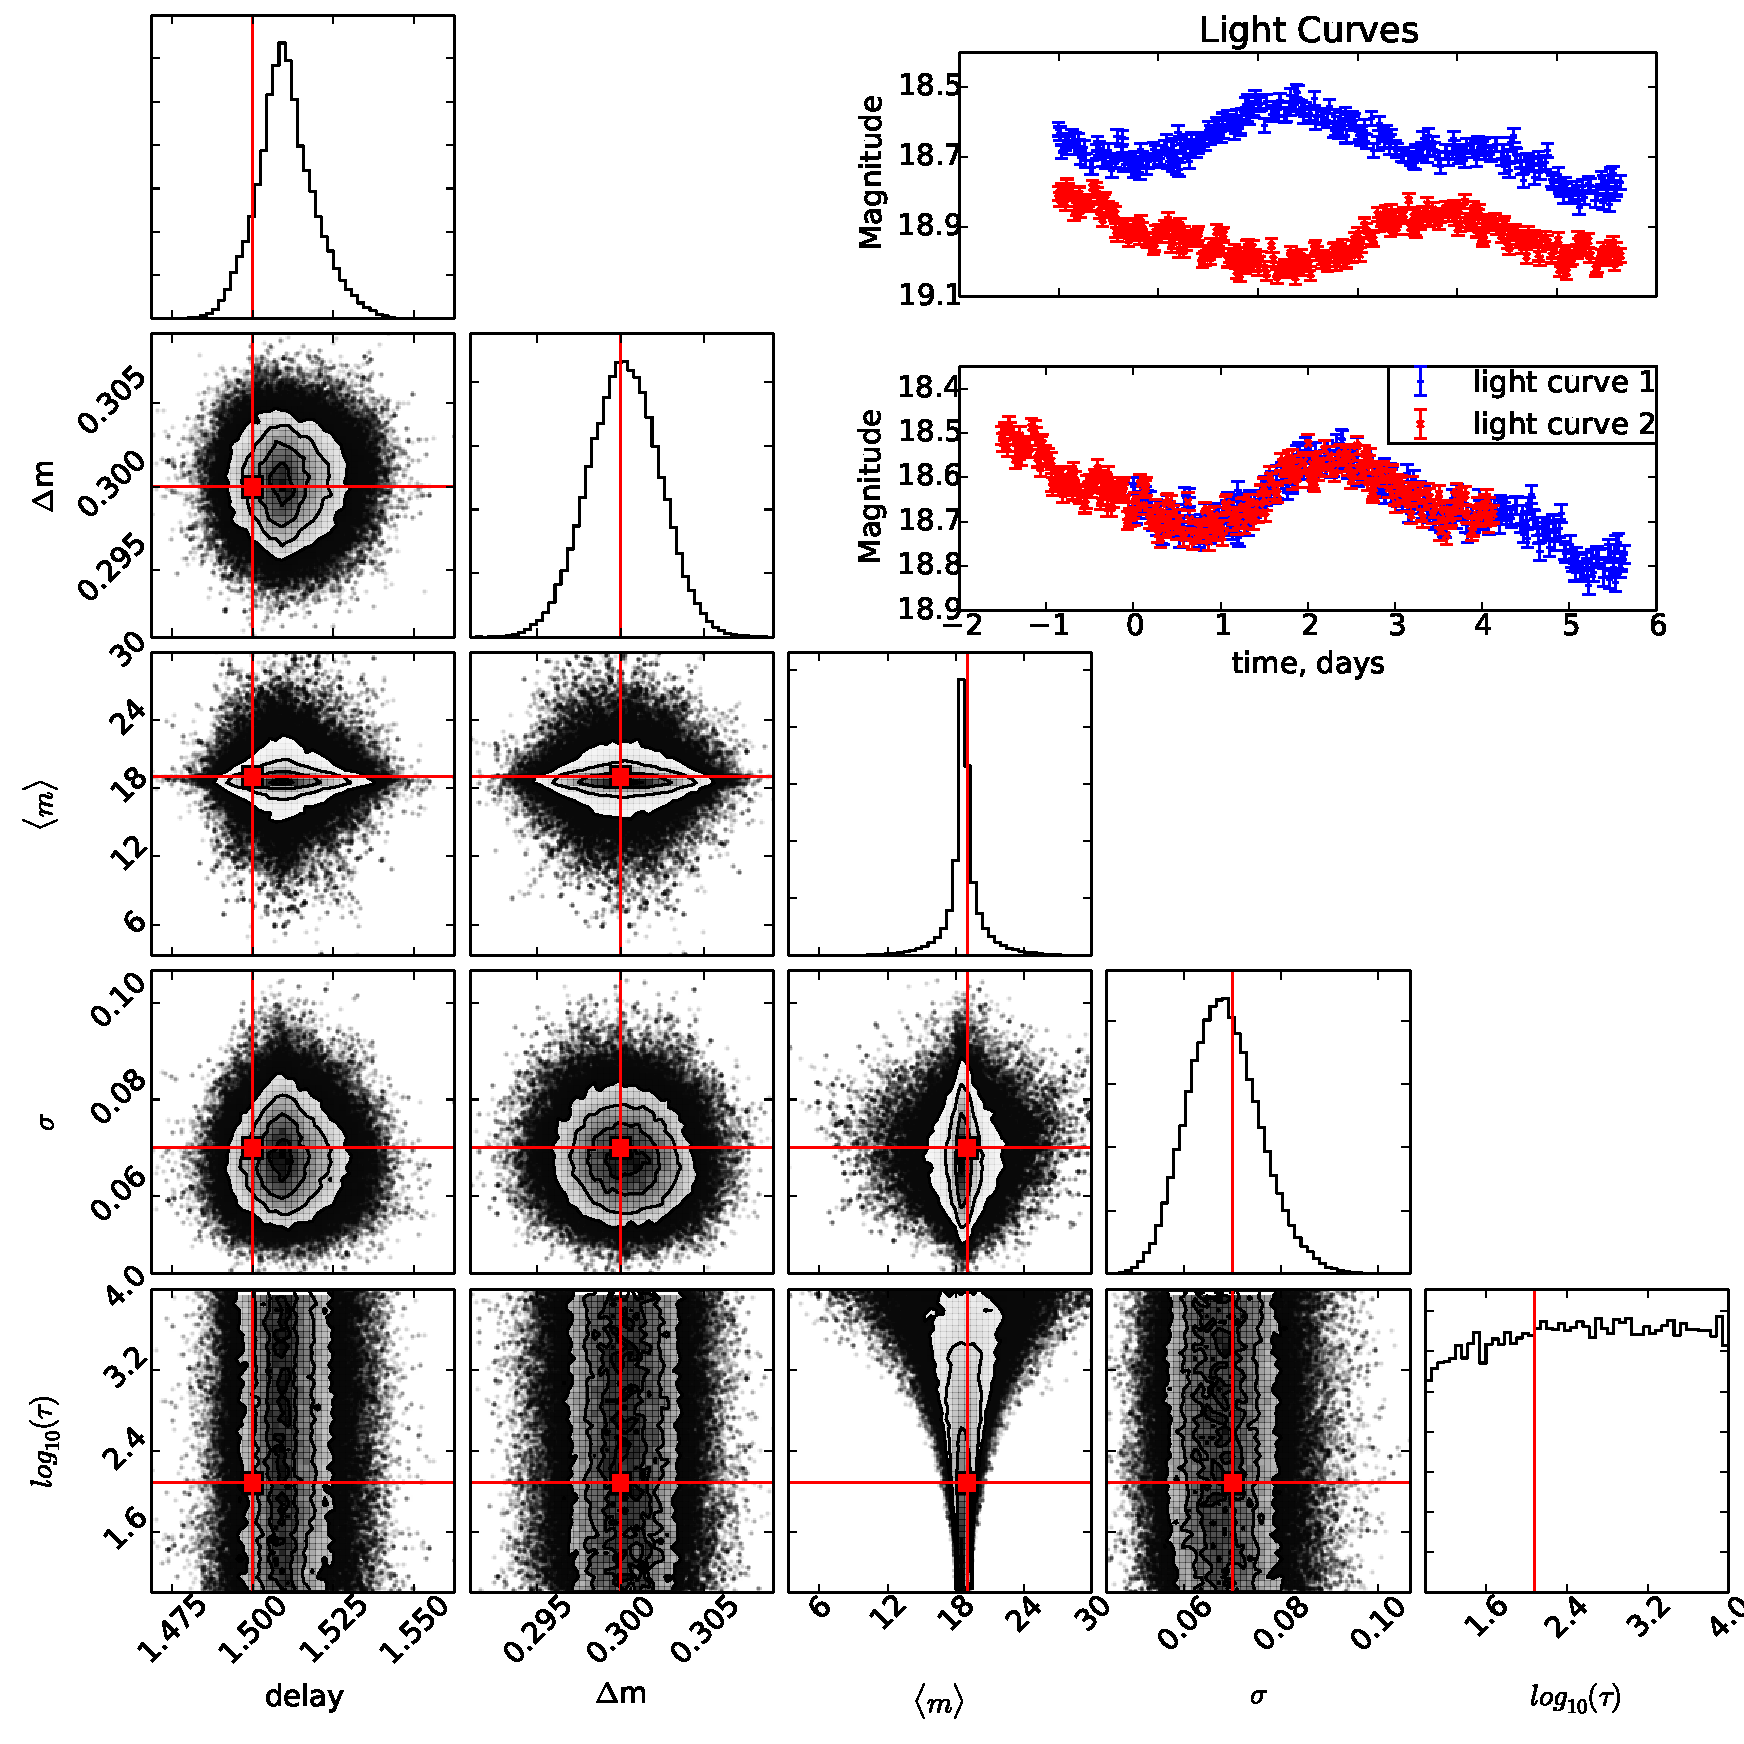
\includegraphics[width=\linewidth]{./triangle_example_2.pdf}
% 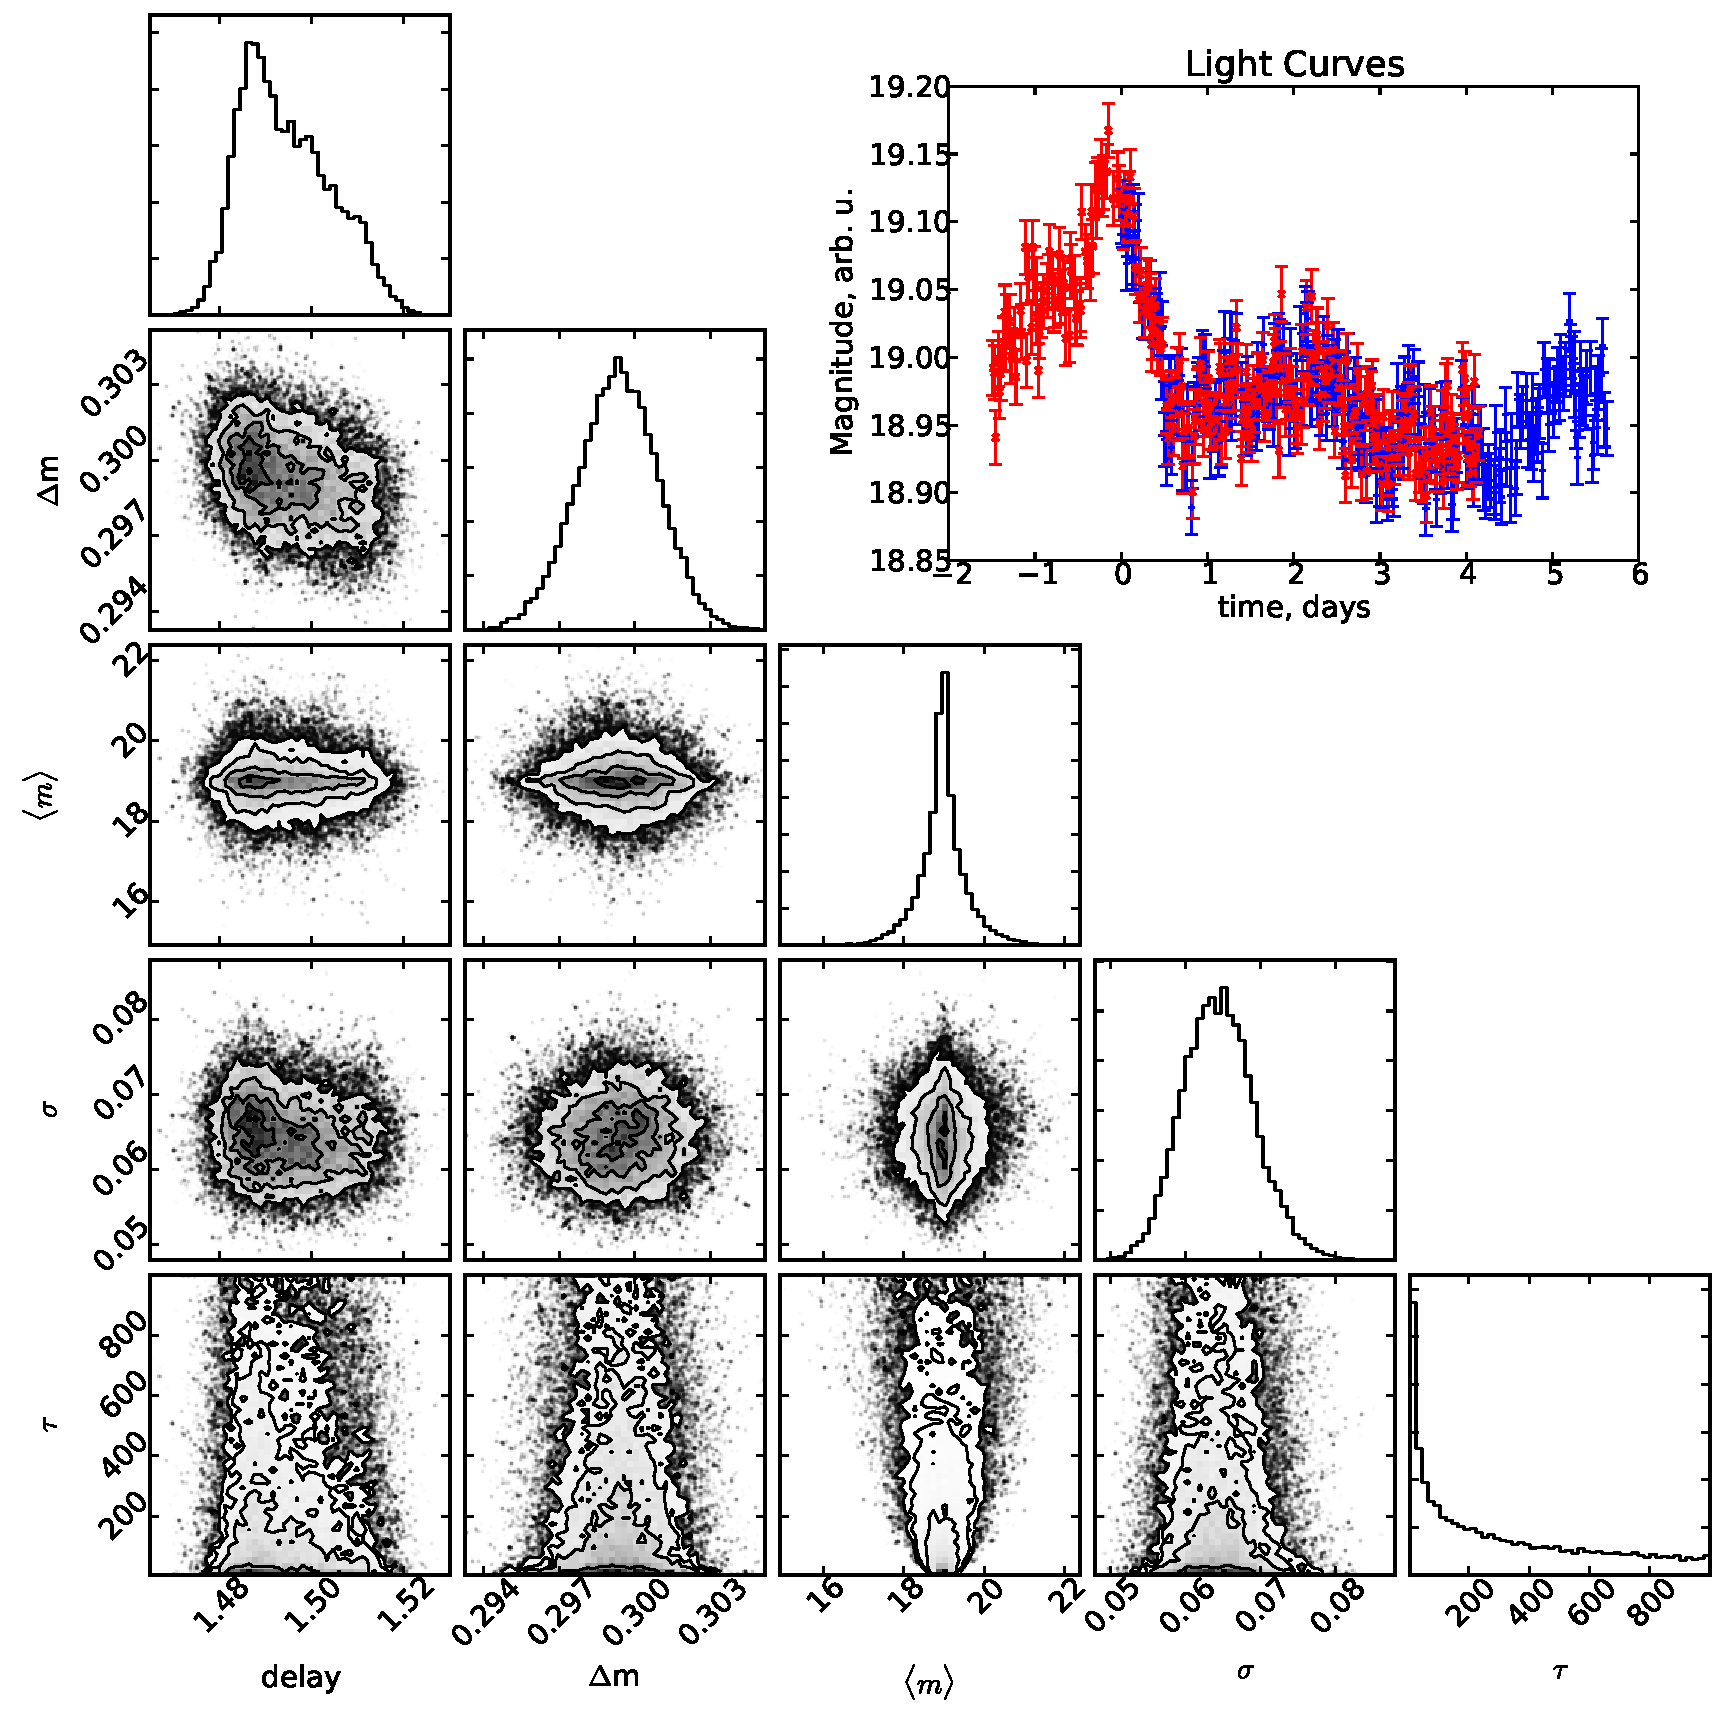
\includegraphics[width=\linewidth]{./triangle_example.pdf}
\caption{
  Markov Chain Monte Carlo (MCMC) results for an example for
  the parameter reconstruction of a light curve and its delayed and
  magnitude offset image. The quasar light curve parameters $\tau$,
  $\sigma$ and $\langle m \rangle$ are estimated under a hypothesis
  value for the delay and $\Delta m$. On the top right the quasar
  light curve (blue) and its delayed magnitude offset image (red) are
  shown with the image delay and magnitude offset corrected from the
  most probable values of the delay and $\Delta m$
  distributions. The quasar light curve parameters are 
  $\langle m \rangle$=19.0~magnitudes, $\sigma$=0.07 mag $day^{-1/2}$
  and $\tau$=121~days. In this example, the observations were modeled
  with a photometric uncertainy of 0.02~magnitudes. Truth values are 
  shown as red lines overlaid on the sampled distributions.}\label{fig:triangle}
\end{center}
\end{figure}

\section{An Experimental Design}\label{sec:experiment}

To test our approach we explore what observational design parameters
would be required to achieve a greater than 90\% probability of
measuring a $1.5$~day time delay, to a combined random and systematic
precision of better than 1.0 hour. To make this exploration more
concrete, we assume space-quality high resolution observations (e.g.\
with the \emph{Hubble} Space Telescope; $HST$), to confidently be able
to assume completely independent non-overlapping photometric
measurements of each image in our notional gravitational lens, and
photometric stability that may be more robustly assumed to be stable
to at least $\sim1\%$.  For the purposes of this setup, we adopt the
$HST$ ``orbit'' as a natural unit of time, which equals
$\sim90$\,minutes.

% {\bf Please update this paragraph to the most final (and ideally the
%   simplest) approach that we ended up taking. The fewer ``post''
% %   processing magical steps we have as part of the process, the better.
%   We can also give some of the technical details on the numbers of
%   walkers, and the burn-in approach that we took, that would be fine.
%   We may also give a sense of how long things took to run on our
%   particular machine, if that would seem useful.}  

In nature, one set of observations may accurately represent our
statistical description of a process, but that set may or may not in
itself contain enough information to allow a clear inference of the
details of the underlying process. To test the efficacy of a planned
experimental design, so we can confidently forecast the probability of
success, an understanding of the likely nature of outlier
measurements, and the performance as a function of the specific
target values for each observational constraint, we generate a large
set of simulated observations drawn from the same observational
characteristics, and do the full inference analysis on each of these.
The results from such a Monte Carlo exploration of an experimental
setup are shown in Figure~\ref{fig:example}, for the set of
observational choices shown in the same Figure. 

The cuts required by for a valid reconstruction are described as follows. 
We fit a Gaussian curve to the distribution of 100 simulation delay results (see Figure~\ref{fig:example}). 
We have found that the python SciPy curve\_fit method, which employs the
Levenberg-Marquardt algorithm, is not driven by outliers. The standard
deviation $\sigma$ from the fit is used to reject reconstruction
results by requiring that a reconstructed delay be within 3$\sigma$ of
the true delay. We also require that the uncertainty in the delay, 
obtained from the posterior distribution of the MCMC process (see the top left 
panel of Figure~\ref{fig:triangle} for an example), to be
within 3$\sigma$ to reject poor reconstructions. We define the success as the 
fraction of light curve delay reconstructions surviving these cuts.

% \begin{table}[htdp]
% \caption{Table of observational parameters.}
% \begin{center}
% \begin{tabular}{lll}
% \hline
% thing & data & description \\
% \hline
% \hline
% stuff & numbers & things \\
% stuff & numbers & things \\
% stuff & numbers & things \\
% \hline
% \end{tabular}
% \end{center}
% \label{tab:example}
% \end{table}



% \begin{figure}[t]
% \begin{center}
% 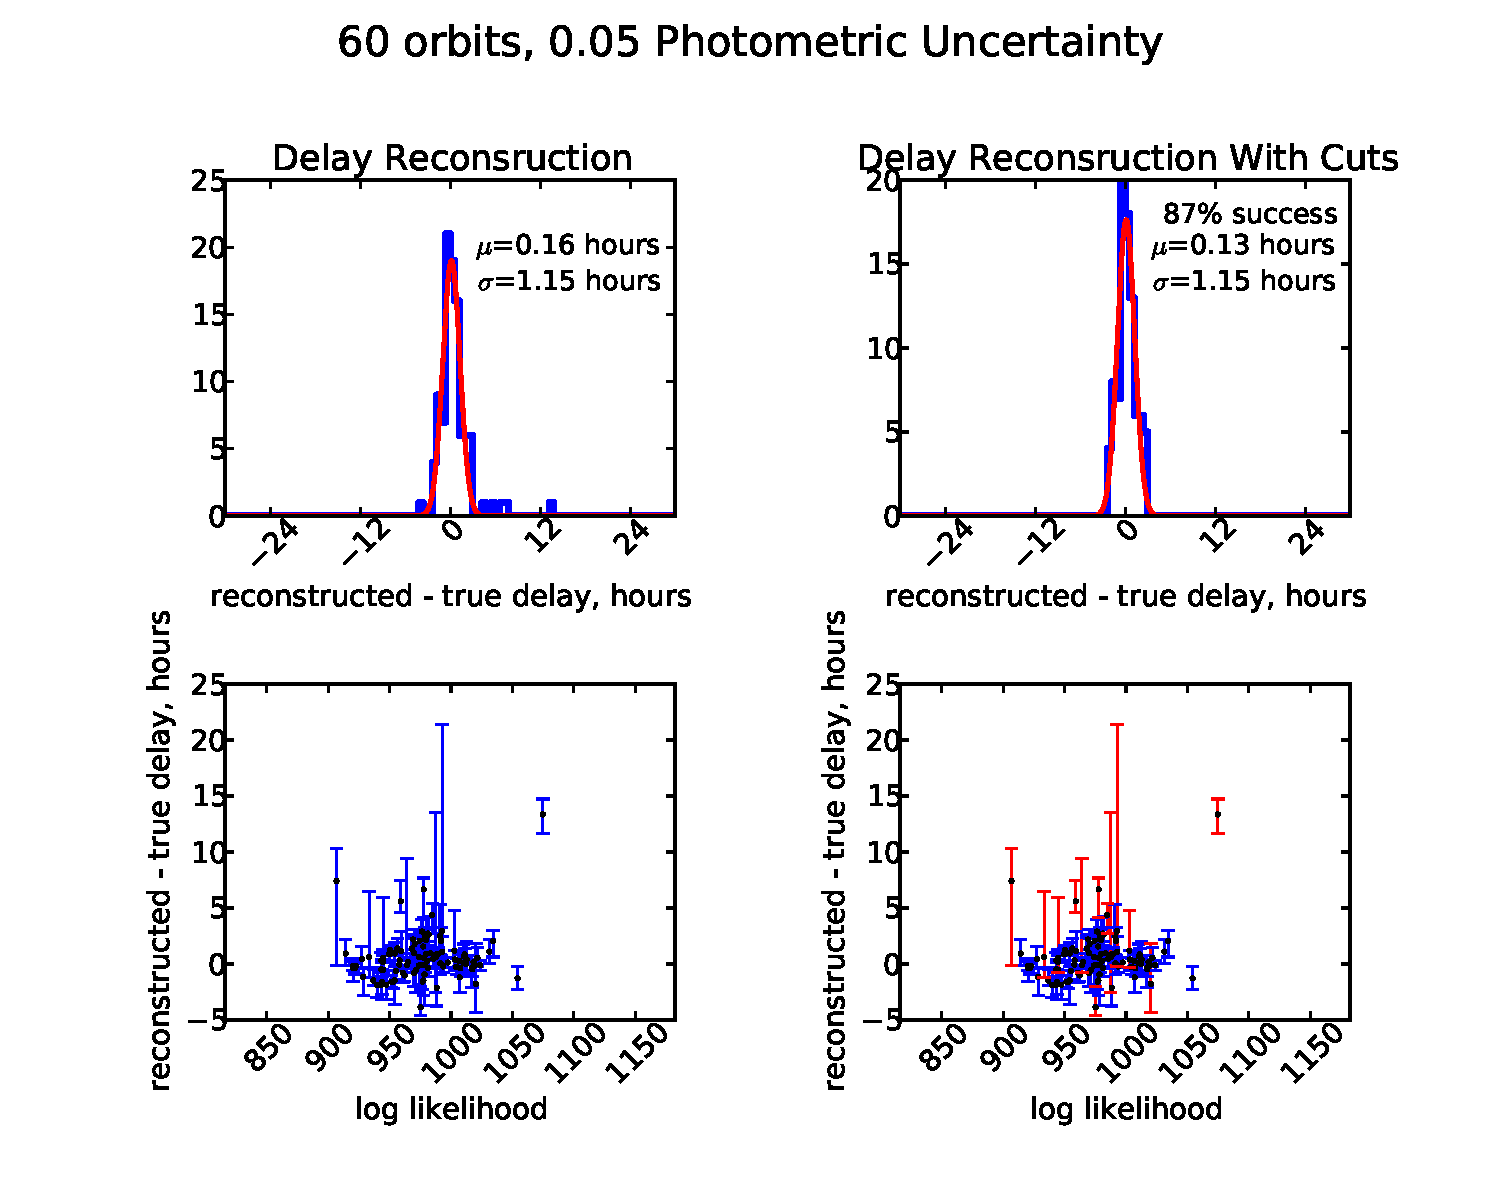
\includegraphics[width=\linewidth]{./ana_ll_example.pdf}
% \caption{The systematic behavior of the reconstruction is
%   characterized using the distribution of 100 reconstructed
%   delays. The example shown here is for 60 orbits and a photometric
%   uncertainty of 0.05 mag. The top left shows a distribution of the
%   results with a Gaussian fit with standard deviation $\sigma$. The
%   bottom left shows the delay residuals, with uncertainties derived
%   from the MCMC analysis, vs. the log-likelihood value of the
%   reconstruction. The bottom left figure shows the same plot with the
%   cuts described in the text. The rejected instances are highlighted
%   in red. The top right plot shows the distribution of delay residuals
%   after the rejected instances have been cut out. In this particular
%   example 13\% of the events did not reconstruct with the fidelity
%   required.}\label{fig:volume}
% \end{center}
% \end{figure}

\begin{figure}[t]
\begin{center}
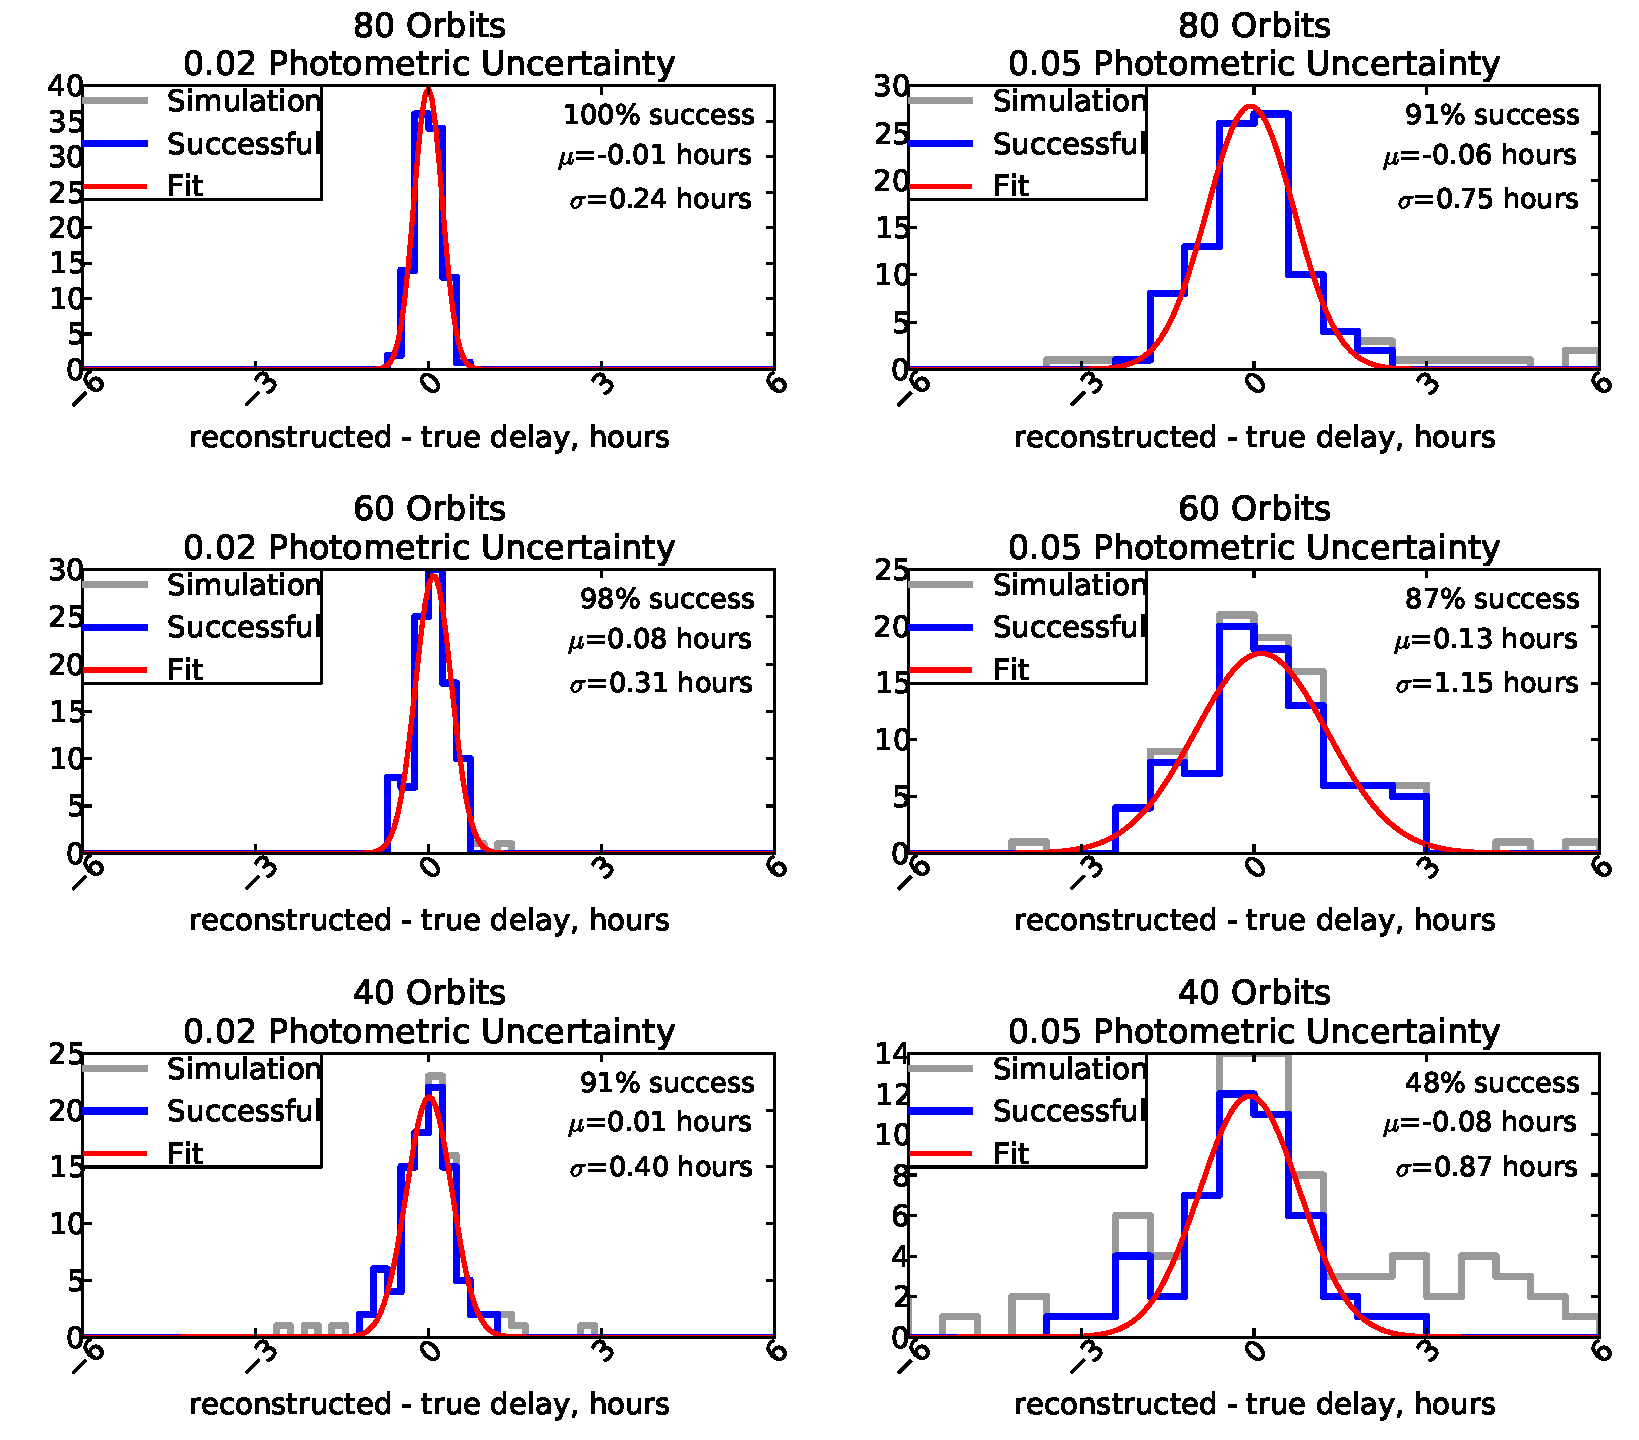
\includegraphics[width=\linewidth]{./systematic_examples.pdf}
\caption{The probability of a successful measurement and resolution
  are shown for several examples of number of orbits and photomoetric
  uncertainty. The delay residuals from the simulations are shown in
  gray. The distribution of successful instances, with the
  requirements described in the text, are shown in blue. A Gaussian
  function is fit to the distribution of successful delay
  reconstructions for a convenient estimate of the final (non-outlier)
  time delay measurement fidelity.}\label{fig:example}
\end{center}
\end{figure}

\begin{figure}[t]
\begin{center}
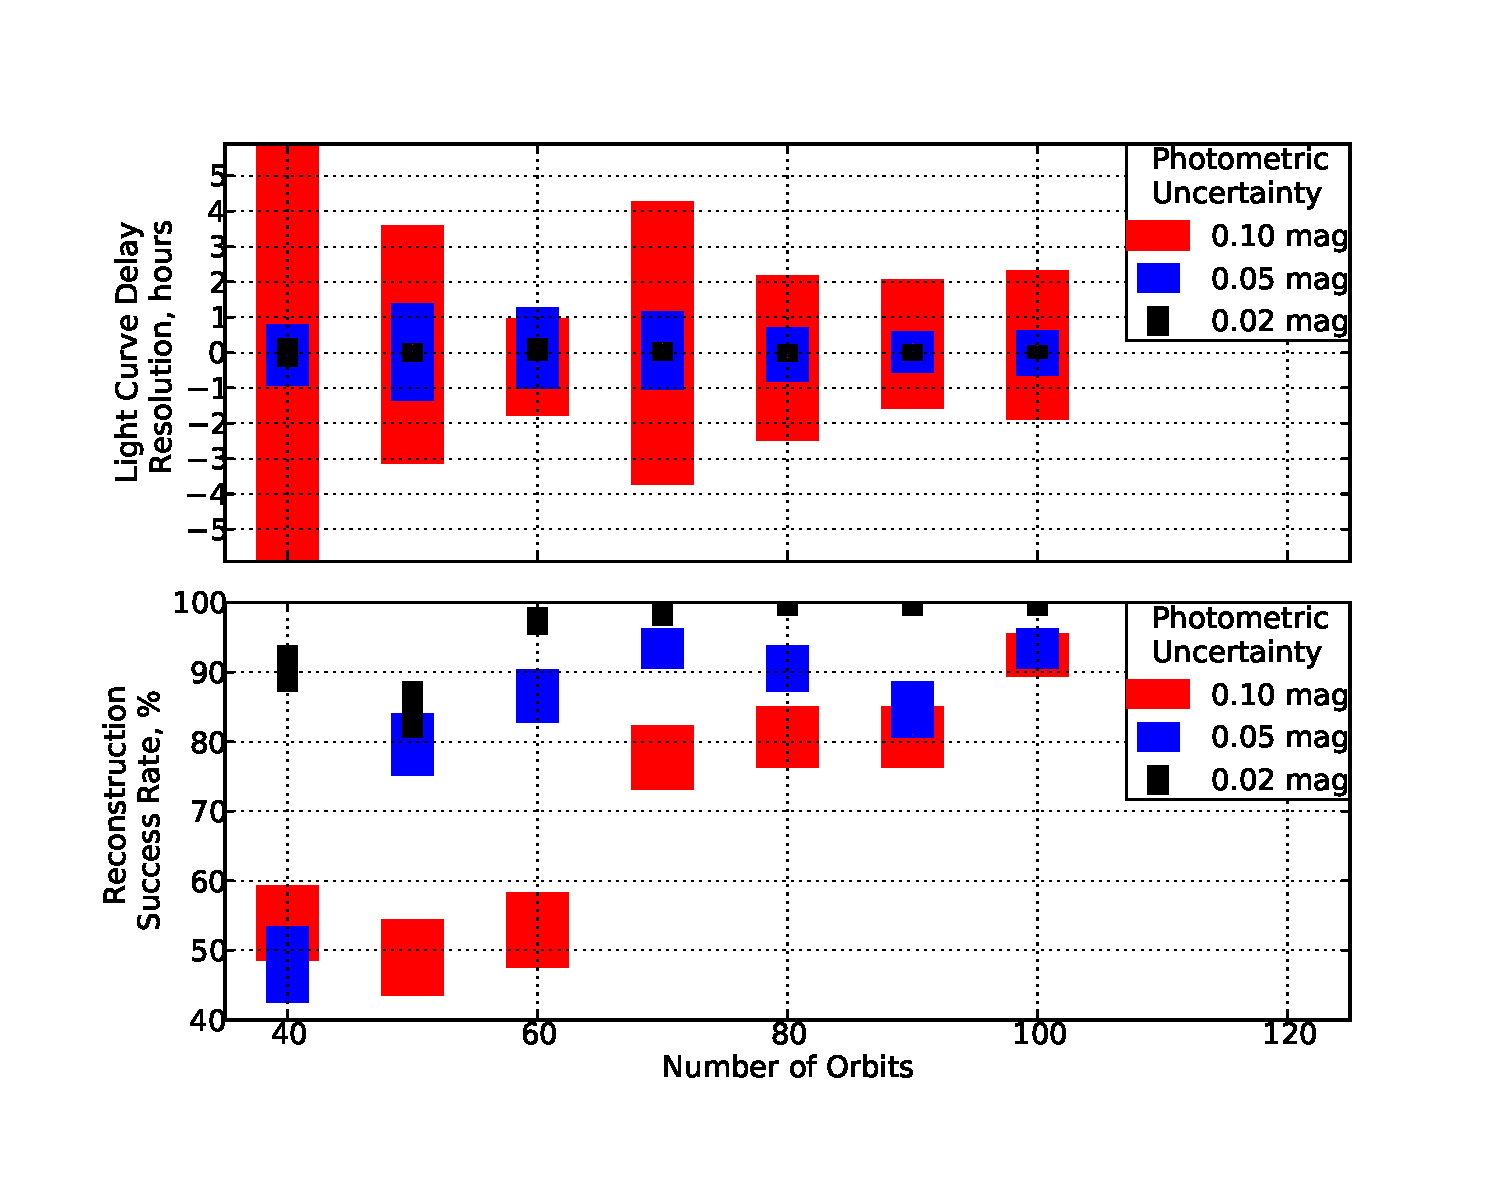
\includegraphics[width=\linewidth]{./systematics_smy.pdf}
\caption{Summary of results for the delay measurement resolution (top
  panel) reconstruction success rate (bottom panel). Photometric
  uncertainties of 0.02~mag result in delay resolutions smaller than
  one day and are down to six hours for 80 orbits and above. Even with
  photometric uncertainties of 0.05~mag, delay resolutions smaller
  that 1~day can be achieved. The reconstruction success is 90\% for
  more than 60 orbits and photometric uncertainties below
  0.05~mag.}\label{fig:summary}
\end{center}
\end{figure}

\section{Discussion and Conclusions}\label{sec:discussion}

We discuss the lessons from our analysis and the process of having
designed an experiment, with an emphasis on the possible pitfalls. The
way that the priors are set up, and carefully establishing enough
burn-in chains in the MCMC process, are important.  For a consistency
check, we can analyze each image's timestream separately as well as
jointly, and compare derived values for the light curve structure
parameters. We have also implicitly assumed that the photometric
measurement uncertainties are uncorrelated, which may not be the case
for e.g.\ deconvolved ground-based observations. However, it is straightforward
to incorporate such covariances in our analysis. 

The setup in Section~\ref{sec:experiment}, by concentrating on a
relatively short intrinsic time delay, largely avoids the effect that
stochastic microlensing variations in one or both of the images would
have. This is a variational component that can be included with
additional parametrizations in our model, and will be the topic of
future work. Isolating and characterizing the microlensing signal in
long-term monitoring observations of lenses is important in its own
right, because it can be used as an additional measurement of the
internal smooth dark matter component in lensing galaxies
\citep{Schechter2002a}, as well as a probe for the detailed structure
of the quasar accretion disk \citep[e.g.][]{Morgan2010a}.

The method developed here has been applied to the Time Delay Challenge
exercise (references here; marked there as the ``JPL'' contributor),
which emulates data similar to what is expected from the Large
Synoptic Survey Telescope (LSST).  As those are expected to be
extremely long time-streams (extending to years), microlensing was a
significant element in many of the light curves, which impacted our 
performance. A new ``grander'' time delay challenge is being
discussed, with a focus on achieving absolute precision time delay
measurements that are more on the order of the experimental setup of
Section~\ref{sec:experiment}. 

{\bf Final paragraphs should end with a short discussion of future plans, e.g. OMEGA,
testing the damped random walk model at short time scales with Kepler, etc.}

\acknowledgements

This work was carried out at Jet Propulsion Laboratory, California
Institute of Technology, under a contract with NASA.  We are grateful
for conversations with Francis-Yan Cyr-Racine, Chuck Keeton, and
Frederic Courbin. 

\bibliographystyle{apj}

\bibliography{/Users/leonidas/Dropbox/bibdesk/moustakasbibs}

\end{document}



%\section{Simulating lensed quasar light curves}\label{sec:qlc} 

% Choices for observing campaigns (remember, this is just for straight
% light curves at the moment. )
% 
% Random and systematic, possibility of covariances, and so on.  
% 
% Relative consequences or advantages of ground versus space. 
% 
% Table summarizing the cadence/campaign/uncertainty combinations we adopt in this paper. 
% 
% Figure of sample light curves and reconstructed parameters. 